\documentclass[1p]{elsarticle_modified}
%\bibliographystyle{elsarticle-num}

%\usepackage[colorlinks]{hyperref}
%\usepackage{abbrmath_seonhwa} %\Abb, \Ascr, \Acal ,\Abf, \Afrak
\usepackage{amsfonts}
\usepackage{amssymb}
\usepackage{amsmath}
\usepackage{amsthm}
\usepackage{scalefnt}
\usepackage{amsbsy}
\usepackage{kotex}
\usepackage{caption}
\usepackage{subfig}
\usepackage{color}
\usepackage{graphicx}
\usepackage{xcolor} %% white, black, red, green, blue, cyan, magenta, yellow
\usepackage{float}
\usepackage{setspace}
\usepackage{hyperref}

\usepackage{tikz}
\usetikzlibrary{arrows}

\usepackage{multirow}
\usepackage{array} % fixed length table
\usepackage{hhline}

%%%%%%%%%%%%%%%%%%%%%
\makeatletter
\renewcommand*\env@matrix[1][\arraystretch]{%
	\edef\arraystretch{#1}%
	\hskip -\arraycolsep
	\let\@ifnextchar\new@ifnextchar
	\array{*\c@MaxMatrixCols c}}
\makeatother %https://tex.stackexchange.com/questions/14071/how-can-i-increase-the-line-spacing-in-a-matrix
%%%%%%%%%%%%%%%

\usepackage[normalem]{ulem}

\newcommand{\msout}[1]{\ifmmode\text{\sout{\ensuremath{#1}}}\else\sout{#1}\fi}
%SOURCE: \msout is \stkout macro in https://tex.stackexchange.com/questions/20609/strikeout-in-math-mode

\newcommand{\cancel}[1]{
	\ifmmode
	{\color{red}\msout{#1}}
	\else
	{\color{red}\sout{#1}}
	\fi
}

\newcommand{\add}[1]{
	{\color{blue}\uwave{#1}}
}

\newcommand{\replace}[2]{
	\ifmmode
	{\color{red}\msout{#1}}{\color{blue}\uwave{#2}}
	\else
	{\color{red}\sout{#1}}{\color{blue}\uwave{#2}}
	\fi
}

\newcommand{\Sol}{\mathcal{S}} %segment
\newcommand{\D}{D} %diagram
\newcommand{\A}{\mathcal{A}} %arc


%%%%%%%%%%%%%%%%%%%%%%%%%%%%%5 test

\def\sl{\operatorname{\textup{SL}}(2,\Cbb)}
\def\psl{\operatorname{\textup{PSL}}(2,\Cbb)}
\def\quan{\mkern 1mu \triangleright \mkern 1mu}

\theoremstyle{definition}
\newtheorem{thm}{Theorem}[section]
\newtheorem{prop}[thm]{Proposition}
\newtheorem{lem}[thm]{Lemma}
\newtheorem{ques}[thm]{Question}
\newtheorem{cor}[thm]{Corollary}
\newtheorem{defn}[thm]{Definition}
\newtheorem{exam}[thm]{Example}
\newtheorem{rmk}[thm]{Remark}
\newtheorem{alg}[thm]{Algorithm}

\newcommand{\I}{\sqrt{-1}}
\begin{document}

%\begin{frontmatter}
%
%\title{Boundary parabolic representations of knots up to 8 crossings}
%
%%% Group authors per affiliation:
%\author{Yunhi Cho} 
%\address{Department of Mathematics, University of Seoul, Seoul, Korea}
%\ead{yhcho@uos.ac.kr}
%
%
%\author{Seonhwa Kim} %\fnref{s_kim}}
%\address{Center for Geometry and Physics, Institute for Basic Science, Pohang, 37673, Korea}
%\ead{ryeona17@ibs.re.kr}
%
%\author{Hyuk Kim}
%\address{Department of Mathematical Sciences, Seoul National University, Seoul 08826, Korea}
%\ead{hyukkim@snu.ac.kr}
%
%\author{Seokbeom Yoon}
%\address{Department of Mathematical Sciences, Seoul National University, Seoul, 08826,  Korea}
%\ead{sbyoon15@snu.ac.kr}
%
%\begin{abstract}
%We find all boundary parabolic representation of knots up to 8 crossings.
%
%\end{abstract}
%\begin{keyword}
%    \MSC[2010] 57M25 
%\end{keyword}
%
%\end{frontmatter}

%\linenumbers
%\tableofcontents
%
\newcommand\colored[1]{\textcolor{white}{\rule[-0.35ex]{0.8em}{1.4ex}}\kern-0.8em\color{red} #1}%
%\newcommand\colored[1]{\textcolor{white}{ #1}\kern-2.17ex	\textcolor{white}{ #1}\kern-1.81ex	\textcolor{white}{ #1}\kern-2.15ex\color{red}#1	}

{\Large $\underline{12n_{0677}~(K12n_{0677})}$}

\setlength{\tabcolsep}{10pt}
\renewcommand{\arraystretch}{1.6}
\vspace{1cm}\begin{tabular}{m{100pt}>{\centering\arraybackslash}m{274pt}}
\multirow{5}{120pt}{
	\centering
	\includegraphics[width=112pt]{../../../GIT/diagram.site/Diagrams/png/2766_12n_0677.png}\\
\ \ \ A knot diagram\footnotemark}&
\allowdisplaybreaks
\textbf{Linearized knot diagam} \\
\cline{2-2}
 &
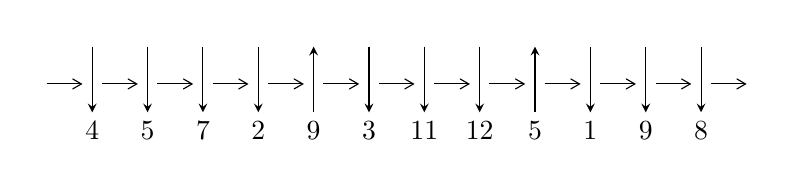
\begin{tikzpicture}[x=20pt, y=17pt]
	% nodes
	\node (C0) at (0, 0) {};
	\node (C1) at (1, 0) {};
	\node (C1U) at (1, +1) {};
	\node (C1D) at (1, -1) {4};

	\node (C2) at (2, 0) {};
	\node (C2U) at (2, +1) {};
	\node (C2D) at (2, -1) {5};

	\node (C3) at (3, 0) {};
	\node (C3U) at (3, +1) {};
	\node (C3D) at (3, -1) {7};

	\node (C4) at (4, 0) {};
	\node (C4U) at (4, +1) {};
	\node (C4D) at (4, -1) {2};

	\node (C5) at (5, 0) {};
	\node (C5U) at (5, +1) {};
	\node (C5D) at (5, -1) {9};

	\node (C6) at (6, 0) {};
	\node (C6U) at (6, +1) {};
	\node (C6D) at (6, -1) {3};

	\node (C7) at (7, 0) {};
	\node (C7U) at (7, +1) {};
	\node (C7D) at (7, -1) {11};

	\node (C8) at (8, 0) {};
	\node (C8U) at (8, +1) {};
	\node (C8D) at (8, -1) {12};

	\node (C9) at (9, 0) {};
	\node (C9U) at (9, +1) {};
	\node (C9D) at (9, -1) {5};

	\node (C10) at (10, 0) {};
	\node (C10U) at (10, +1) {};
	\node (C10D) at (10, -1) {1};

	\node (C11) at (11, 0) {};
	\node (C11U) at (11, +1) {};
	\node (C11D) at (11, -1) {9};

	\node (C12) at (12, 0) {};
	\node (C12U) at (12, +1) {};
	\node (C12D) at (12, -1) {8};
	\node (C13) at (13, 0) {};

	% arrows
	\draw[->,>={angle 60}]
	(C0) edge (C1) (C1) edge (C2) (C2) edge (C3) (C3) edge (C4) (C4) edge (C5) (C5) edge (C6) (C6) edge (C7) (C7) edge (C8) (C8) edge (C9) (C9) edge (C10) (C10) edge (C11) (C11) edge (C12) (C12) edge (C13) ;	\draw[->,>=stealth]
	(C1U) edge (C1D) (C2U) edge (C2D) (C3U) edge (C3D) (C4U) edge (C4D) (C5D) edge (C5U) (C6U) edge (C6D) (C7U) edge (C7D) (C8U) edge (C8D) (C9D) edge (C9U) (C10U) edge (C10D) (C11U) edge (C11D) (C12U) edge (C12D) ;
	\end{tikzpicture} \\
\hhline{~~} \\& 
\textbf{Solving Sequence} \\ \cline{2-2} 
 &
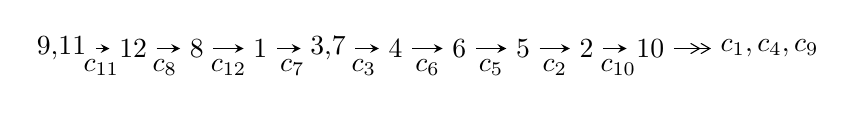
\begin{tikzpicture}[x=23pt, y=7pt]
	% node
	\node (A0) at (-1/8, 0) {9,11};
	\node (A1) at (1, 0) {12};
	\node (A2) at (2, 0) {8};
	\node (A3) at (3, 0) {1};
	\node (A4) at (65/16, 0) {3,7};
	\node (A5) at (41/8, 0) {4};
	\node (A6) at (49/8, 0) {6};
	\node (A7) at (57/8, 0) {5};
	\node (A8) at (65/8, 0) {2};
	\node (A9) at (73/8, 0) {10};
	\node (C1) at (1/2, -1) {$c_{11}$};
	\node (C2) at (3/2, -1) {$c_{8}$};
	\node (C3) at (5/2, -1) {$c_{12}$};
	\node (C4) at (7/2, -1) {$c_{7}$};
	\node (C5) at (37/8, -1) {$c_{3}$};
	\node (C6) at (45/8, -1) {$c_{6}$};
	\node (C7) at (53/8, -1) {$c_{5}$};
	\node (C8) at (61/8, -1) {$c_{2}$};
	\node (C9) at (69/8, -1) {$c_{10}$};
	\node (A10) at (11, 0) {$c_{1},c_{4},c_{9}$};

	% edge
	\draw[->,>=stealth]	
	(A0) edge (A1) (A1) edge (A2) (A2) edge (A3) (A3) edge (A4) (A4) edge (A5) (A5) edge (A6) (A6) edge (A7) (A7) edge (A8) (A8) edge (A9) ;
	\draw[->>,>={angle 60}]	
	(A9) edge (A10);
\end{tikzpicture} \\ 

\end{tabular} \\

\footnotetext{
The image of knot diagram is generated by the software ``\textbf{Draw programme}" developed by Andrew Bartholomew(\url{http://www.layer8.co.uk/maths/draw/index.htm\#Running-draw}), where we modified some parts for our purpose(\url{https://github.com/CATsTAILs/LinksPainter}).
}\phantom \\ \newline 
\centering \textbf{Ideals for irreducible components\footnotemark of $X_{\text{par}}$} 
 
\begin{align*}
I^u_{1}&=\langle 
84729282499200 u^{49}+3758065856672058 u^{48}+\cdots+6852922461300829 b-6852284696559709,\\
\phantom{I^u_{1}}&\phantom{= \langle  }-6.85291\times10^{15} u^{49}+2.05586\times10^{16} u^{48}+\cdots+1.37058\times10^{16} a+9.44180\times10^{16},\\
\phantom{I^u_{1}}&\phantom{= \langle  }u^{50}-3 u^{49}+\cdots-14 u+1\rangle \\
I^u_{2}&=\langle 
2 a u+u^2+b+u+1,\;- u^2 a+a^2- u^2- a- u-2,\;u^3+u^2+2 u+1\rangle \\
\\
\end{align*}
\raggedright * 2 irreducible components of $\dim_{\mathbb{C}}=0$, with total 56 representations.\\
\footnotetext{All coefficients of polynomials are rational numbers. But the coefficients are sometimes approximated in decimal forms when there is not enough margin.}
\newpage
\renewcommand{\arraystretch}{1}
\centering \section*{I. $I^u_{1}= \langle 8.47\times10^{13} u^{49}+3.76\times10^{15} u^{48}+\cdots+6.85\times10^{15} b-6.85\times10^{15},\;-6.85\times10^{15} u^{49}+2.06\times10^{16} u^{48}+\cdots+1.37\times10^{16} a+9.44\times10^{16},\;u^{50}-3 u^{49}+\cdots-14 u+1 \rangle$}
\flushleft \textbf{(i) Arc colorings}\\
\begin{tabular}{m{7pt} m{180pt} m{7pt} m{180pt} }
\flushright $a_{9}=$&$\begin{pmatrix}0\\u\end{pmatrix}$ \\
\flushright $a_{11}=$&$\begin{pmatrix}1\\0\end{pmatrix}$ \\
\flushright $a_{12}=$&$\begin{pmatrix}1\\u^2\end{pmatrix}$ \\
\flushright $a_{8}=$&$\begin{pmatrix}u\\u^3+u\end{pmatrix}$ \\
\flushright $a_{1}=$&$\begin{pmatrix}u^2+1\\u^4+2 u^2\end{pmatrix}$ \\
\flushright $a_{3}=$&$\begin{pmatrix}0.499999 u^{49}-1.49999 u^{48}+\cdots+15.0256 u-6.88889\\-0.0123640 u^{49}-0.548389 u^{48}+\cdots-3.33203 u+0.999907\end{pmatrix}$ \\
\flushright $a_{7}=$&$\begin{pmatrix}u^3+2 u\\u^3+u\end{pmatrix}$ \\
\flushright $a_{4}=$&$\begin{pmatrix}0.666682 u^{49}-2.00117 u^{48}+\cdots+26.2921 u-7.92593\\-0.00103128 u^{49}+0.120354 u^{48}+\cdots-2.70359 u+0.833325\end{pmatrix}$ \\
\flushright $a_{6}=$&$\begin{pmatrix}-0.333328 u^{49}+0.999541 u^{48}+\cdots+1.63220 u+3.29630\\-0.0354893 u^{49}+1.92137 u^{48}+\cdots-2.80779 u-0.167168\end{pmatrix}$ \\
\flushright $a_{5}=$&$\begin{pmatrix}-0.333328 u^{49}+0.999541 u^{48}+\cdots+1.63220 u+3.29630\\-0.00783089 u^{49}+0.919108 u^{48}+\cdots-2.48066 u-0.166726\end{pmatrix}$ \\
\flushright $a_{2}=$&$\begin{pmatrix}0.166654 u^{49}-0.499067 u^{48}+\cdots+15.7612 u-4.48148\\0.00329781 u^{49}+0.613395 u^{48}+\cdots+0.629281 u+0.333358\end{pmatrix}$ \\
\flushright $a_{10}=$&$\begin{pmatrix}- u^6-3 u^4-2 u^2+1\\- u^8-4 u^6-4 u^4\end{pmatrix}$\\&\end{tabular}
\flushleft \textbf{(ii) Obstruction class $= -1$}\\~\\
\flushleft \textbf{(iii) Cusp Shapes $= \frac{5330467839288029}{6852922461300829} u^{49}-\frac{25189087260468945}{13705844922601658} u^{48}+\cdots+\frac{266207119693174765}{13705844922601658} u-\frac{140924841106764001}{13705844922601658}$}\\~\\
\newpage\renewcommand{\arraystretch}{1}
\flushleft \textbf{(iv) u-Polynomials at the component}\newline \\
\begin{tabular}{m{50pt}|m{274pt}}
Crossings & \hspace{64pt}u-Polynomials at each crossing \\
\hline $$\begin{aligned}c_{1},c_{2},c_{4}\end{aligned}$$&$\begin{aligned}
&u^{50}-4 u^{49}+\cdots+11 u+1
\end{aligned}$\\
\hline $$\begin{aligned}c_{3},c_{6}\end{aligned}$$&$\begin{aligned}
&u^{50}+4 u^{49}+\cdots- u+1
\end{aligned}$\\
\hline $$\begin{aligned}c_{5},c_{9}\end{aligned}$$&$\begin{aligned}
&u^{50}-3 u^{49}+\cdots+32 u+64
\end{aligned}$\\
\hline $$\begin{aligned}c_{7}\end{aligned}$$&$\begin{aligned}
&u^{50}+3 u^{49}+\cdots-12700 u+977
\end{aligned}$\\
\hline $$\begin{aligned}c_{8},c_{11},c_{12}\end{aligned}$$&$\begin{aligned}
&u^{50}-3 u^{49}+\cdots-14 u+1
\end{aligned}$\\
\hline $$\begin{aligned}c_{10}\end{aligned}$$&$\begin{aligned}
&u^{50}-9 u^{49}+\cdots+13688 u+209
\end{aligned}$\\
\hline
\end{tabular}\\~\\
\newpage\renewcommand{\arraystretch}{1}
\flushleft \textbf{(v) Riley Polynomials at the component}\newline \\
\begin{tabular}{m{50pt}|m{274pt}}
Crossings & \hspace{64pt}Riley Polynomials at each crossing \\
\hline $$\begin{aligned}c_{1},c_{2},c_{4}\end{aligned}$$&$\begin{aligned}
&y^{50}-40 y^{49}+\cdots-19 y+1
\end{aligned}$\\
\hline $$\begin{aligned}c_{3},c_{6}\end{aligned}$$&$\begin{aligned}
&y^{50}-12 y^{49}+\cdots-19 y+1
\end{aligned}$\\
\hline $$\begin{aligned}c_{5},c_{9}\end{aligned}$$&$\begin{aligned}
&y^{50}-35 y^{49}+\cdots-82944 y+4096
\end{aligned}$\\
\hline $$\begin{aligned}c_{7}\end{aligned}$$&$\begin{aligned}
&y^{50}+11 y^{49}+\cdots-129195550 y+954529
\end{aligned}$\\
\hline $$\begin{aligned}c_{8},c_{11},c_{12}\end{aligned}$$&$\begin{aligned}
&y^{50}+47 y^{49}+\cdots-150 y+1
\end{aligned}$\\
\hline $$\begin{aligned}c_{10}\end{aligned}$$&$\begin{aligned}
&y^{50}+31 y^{49}+\cdots-210039934 y+43681
\end{aligned}$\\
\hline
\end{tabular}\\~\\
\newpage\flushleft \textbf{(vi) Complex Volumes and Cusp Shapes}
$$\begin{array}{c|c|c}  
\text{Solutions to }I^u_{1}& \I (\text{vol} + \sqrt{-1}CS) & \text{Cusp shape}\\
 \hline 
\begin{aligned}
u &= \phantom{-}0.552389 + 0.742281 I \\
a &= \phantom{-}0.58850 + 1.59488 I \\
b &= -0.405792 + 0.376362 I\end{aligned}
 & \phantom{-}0.54313 + 5.94487 I & -9.08850 - 3.35912 I \\ \hline\begin{aligned}
u &= \phantom{-}0.552389 - 0.742281 I \\
a &= \phantom{-}0.58850 - 1.59488 I \\
b &= -0.405792 - 0.376362 I\end{aligned}
 & \phantom{-}0.54313 - 5.94487 I & -9.08850 + 3.35912 I \\ \hline\begin{aligned}
u &= -0.922692\phantom{ +0.000000I} \\
a &= -1.08212\phantom{ +0.000000I} \\
b &= -0.943183\phantom{ +0.000000I}\end{aligned}
 & -5.06588\phantom{ +0.000000I} & -21.9910\phantom{ +0.000000I} \\ \hline\begin{aligned}
u &= -0.749534 + 0.478843 I \\
a &= \phantom{-}0.202016 - 0.272595 I \\
b &= \phantom{-}0.365555 - 0.028774 I\end{aligned}
 & -4.15396 + 2.45065 I & -18.0240 - 7.7083 I \\ \hline\begin{aligned}
u &= -0.749534 - 0.478843 I \\
a &= \phantom{-}0.202016 + 0.272595 I \\
b &= \phantom{-}0.365555 + 0.028774 I\end{aligned}
 & -4.15396 - 2.45065 I & -18.0240 + 7.7083 I \\ \hline\begin{aligned}
u &= \phantom{-}0.790702 + 0.343009 I \\
a &= \phantom{-}1.63606 + 1.17395 I \\
b &= \phantom{-}1.55555 + 0.92027 I\end{aligned}
 & -0.76132 - 10.59360 I & -11.03214 + 7.66029 I \\ \hline\begin{aligned}
u &= \phantom{-}0.790702 - 0.343009 I \\
a &= \phantom{-}1.63606 - 1.17395 I \\
b &= \phantom{-}1.55555 - 0.92027 I\end{aligned}
 & -0.76132 + 10.59360 I & -11.03214 - 7.66029 I \\ \hline\begin{aligned}
u &= \phantom{-}0.702274 + 0.393042 I \\
a &= -1.31621 - 1.35430 I \\
b &= -1.36162 - 0.89962 I\end{aligned}
 & \phantom{-}3.75899 - 5.49083 I & -7.01323 + 5.78466 I \\ \hline\begin{aligned}
u &= \phantom{-}0.702274 - 0.393042 I \\
a &= -1.31621 + 1.35430 I \\
b &= -1.36162 + 0.89962 I\end{aligned}
 & \phantom{-}3.75899 + 5.49083 I & -7.01323 - 5.78466 I \\ \hline\begin{aligned}
u &= \phantom{-}0.566166 + 0.558111 I \\
a &= -0.90619 - 1.55455 I \\
b &= -0.020776 - 0.271583 I\end{aligned}
 & \phantom{-}4.38215 + 1.22744 I & -5.15353 + 0.43980 I\\
 \hline 
 \end{array}$$\newpage$$\begin{array}{c|c|c}  
\text{Solutions to }I^u_{1}& \I (\text{vol} + \sqrt{-1}CS) & \text{Cusp shape}\\
 \hline 
\begin{aligned}
u &= \phantom{-}0.566166 - 0.558111 I \\
a &= -0.90619 + 1.55455 I \\
b &= -0.020776 + 0.271583 I\end{aligned}
 & \phantom{-}4.38215 - 1.22744 I & -5.15353 - 0.43980 I \\ \hline\begin{aligned}
u &= -0.120712 + 1.229850 I \\
a &= \phantom{-}1.45598 + 0.19323 I \\
b &= \phantom{-}0.507473 - 0.965365 I\end{aligned}
 & \phantom{-}0.54799 + 1.96970 I & \phantom{-0.000000 } 0 \\ \hline\begin{aligned}
u &= -0.120712 - 1.229850 I \\
a &= \phantom{-}1.45598 - 0.19323 I \\
b &= \phantom{-}0.507473 + 0.965365 I\end{aligned}
 & \phantom{-}0.54799 - 1.96970 I & \phantom{-0.000000 } 0 \\ \hline\begin{aligned}
u &= -0.457079 + 1.168010 I \\
a &= \phantom{-}0.722675 + 0.578522 I \\
b &= \phantom{-}0.755050 - 0.558234 I\end{aligned}
 & -1.48101 + 4.89320 I & \phantom{-0.000000 } 0 \\ \hline\begin{aligned}
u &= -0.457079 - 1.168010 I \\
a &= \phantom{-}0.722675 - 0.578522 I \\
b &= \phantom{-}0.755050 + 0.558234 I\end{aligned}
 & -1.48101 - 4.89320 I & \phantom{-0.000000 } 0 \\ \hline\begin{aligned}
u &= \phantom{-}0.623208 + 0.370284 I \\
a &= \phantom{-}1.11093 + 1.42613 I \\
b &= \phantom{-}0.450819 + 0.112665 I\end{aligned}
 & \phantom{-}0.00046 - 3.40676 I & -9.23836 + 4.55497 I \\ \hline\begin{aligned}
u &= \phantom{-}0.623208 - 0.370284 I \\
a &= \phantom{-}1.11093 - 1.42613 I \\
b &= \phantom{-}0.450819 - 0.112665 I\end{aligned}
 & \phantom{-}0.00046 + 3.40676 I & -9.23836 - 4.55497 I \\ \hline\begin{aligned}
u &= -0.024870 + 1.281810 I \\
a &= \phantom{-}0.558643 - 0.077771 I \\
b &= -0.47247 - 2.22216 I\end{aligned}
 & \phantom{-}2.27889 + 0.01971 I & \phantom{-0.000000 } 0 \\ \hline\begin{aligned}
u &= -0.024870 - 1.281810 I \\
a &= \phantom{-}0.558643 + 0.077771 I \\
b &= -0.47247 + 2.22216 I\end{aligned}
 & \phantom{-}2.27889 - 0.01971 I & \phantom{-0.000000 } 0 \\ \hline\begin{aligned}
u &= -0.239006 + 1.260440 I \\
a &= -0.861709 - 0.739108 I \\
b &= -1.15757 + 1.31290 I\end{aligned}
 & \phantom{-}2.34625 + 3.21609 I & \phantom{-0.000000 } 0\\
 \hline 
 \end{array}$$\newpage$$\begin{array}{c|c|c}  
\text{Solutions to }I^u_{1}& \I (\text{vol} + \sqrt{-1}CS) & \text{Cusp shape}\\
 \hline 
\begin{aligned}
u &= -0.239006 - 1.260440 I \\
a &= -0.861709 + 0.739108 I \\
b &= -1.15757 - 1.31290 I\end{aligned}
 & \phantom{-}2.34625 - 3.21609 I & \phantom{-0.000000 } 0 \\ \hline\begin{aligned}
u &= \phantom{-}0.149426 + 1.300560 I \\
a &= \phantom{-}0.0642609 - 0.0722773 I \\
b &= \phantom{-}1.63464 + 2.09669 I\end{aligned}
 & -5.69465 - 2.27909 I & \phantom{-0.000000 } 0 \\ \hline\begin{aligned}
u &= \phantom{-}0.149426 - 1.300560 I \\
a &= \phantom{-}0.0642609 + 0.0722773 I \\
b &= \phantom{-}1.63464 - 2.09669 I\end{aligned}
 & -5.69465 + 2.27909 I & \phantom{-0.000000 } 0 \\ \hline\begin{aligned}
u &= \phantom{-}0.535241 + 0.419966 I \\
a &= \phantom{-}0.82919 + 1.50246 I \\
b &= \phantom{-}1.147110 + 0.719409 I\end{aligned}
 & \phantom{-}0.319873 - 0.282575 I & -8.47740 + 2.84929 I \\ \hline\begin{aligned}
u &= \phantom{-}0.535241 - 0.419966 I \\
a &= \phantom{-}0.82919 - 1.50246 I \\
b &= \phantom{-}1.147110 - 0.719409 I\end{aligned}
 & \phantom{-}0.319873 + 0.282575 I & -8.47740 - 2.84929 I \\ \hline\begin{aligned}
u &= -0.203499 + 1.334990 I \\
a &= -2.06609 + 0.25372 I \\
b &= -0.87123 + 3.23217 I\end{aligned}
 & \phantom{-}1.75099 + 3.13920 I & \phantom{-0.000000 } 0 \\ \hline\begin{aligned}
u &= -0.203499 - 1.334990 I \\
a &= -2.06609 - 0.25372 I \\
b &= -0.87123 - 3.23217 I\end{aligned}
 & \phantom{-}1.75099 - 3.13920 I & \phantom{-0.000000 } 0 \\ \hline\begin{aligned}
u &= -0.646196\phantom{ +0.000000I} \\
a &= \phantom{-}1.77141\phantom{ +0.000000I} \\
b &= \phantom{-}1.30808\phantom{ +0.000000I}\end{aligned}
 & -1.56699\phantom{ +0.000000I} & -3.89440\phantom{ +0.000000I} \\ \hline\begin{aligned}
u &= -0.16539 + 1.41406 I \\
a &= -0.381243 + 0.117701 I \\
b &= \phantom{-}0.345250 - 0.188328 I\end{aligned}
 & \phantom{-}4.73635 + 3.24367 I & \phantom{-0.000000 } 0 \\ \hline\begin{aligned}
u &= -0.16539 - 1.41406 I \\
a &= -0.381243 - 0.117701 I \\
b &= \phantom{-}0.345250 + 0.188328 I\end{aligned}
 & \phantom{-}4.73635 - 3.24367 I & \phantom{-0.000000 } 0\\
 \hline 
 \end{array}$$\newpage$$\begin{array}{c|c|c}  
\text{Solutions to }I^u_{1}& \I (\text{vol} + \sqrt{-1}CS) & \text{Cusp shape}\\
 \hline 
\begin{aligned}
u &= -0.545177 + 0.098559 I \\
a &= -0.20103 - 4.61567 I \\
b &= -0.12303 - 2.25640 I\end{aligned}
 & -2.79473 + 0.42156 I & -9.5718 + 13.6793 I \\ \hline\begin{aligned}
u &= -0.545177 - 0.098559 I \\
a &= -0.20103 + 4.61567 I \\
b &= -0.12303 + 2.25640 I\end{aligned}
 & -2.79473 - 0.42156 I & -9.5718 - 13.6793 I \\ \hline\begin{aligned}
u &= \phantom{-}0.20588 + 1.44689 I \\
a &= -0.759687 - 0.164512 I \\
b &= -1.97063 - 2.49195 I\end{aligned}
 & \phantom{-}6.28981 - 3.04185 I & \phantom{-0.000000 } 0 \\ \hline\begin{aligned}
u &= \phantom{-}0.20588 - 1.44689 I \\
a &= -0.759687 + 0.164512 I \\
b &= -1.97063 + 2.49195 I\end{aligned}
 & \phantom{-}6.28981 + 3.04185 I & \phantom{-0.000000 } 0 \\ \hline\begin{aligned}
u &= \phantom{-}0.23659 + 1.44426 I \\
a &= -0.896231 - 0.085608 I \\
b &= -1.88095 - 0.27769 I\end{aligned}
 & \phantom{-}5.83118 - 6.56630 I & \phantom{-0.000000 } 0 \\ \hline\begin{aligned}
u &= \phantom{-}0.23659 - 1.44426 I \\
a &= -0.896231 + 0.085608 I \\
b &= -1.88095 + 0.27769 I\end{aligned}
 & \phantom{-}5.83118 + 6.56630 I & \phantom{-0.000000 } 0 \\ \hline\begin{aligned}
u &= \phantom{-}0.26311 + 1.46153 I \\
a &= \phantom{-}1.048660 - 0.063993 I \\
b &= \phantom{-}2.20151 + 2.19868 I\end{aligned}
 & \phantom{-}9.72958 - 9.01297 I & \phantom{-0.000000 } 0 \\ \hline\begin{aligned}
u &= \phantom{-}0.26311 - 1.46153 I \\
a &= \phantom{-}1.048660 + 0.063993 I \\
b &= \phantom{-}2.20151 - 2.19868 I\end{aligned}
 & \phantom{-}9.72958 + 9.01297 I & \phantom{-0.000000 } 0 \\ \hline\begin{aligned}
u &= \phantom{-}0.30795 + 1.45297 I \\
a &= -1.163440 + 0.334790 I \\
b &= -2.26238 - 1.86908 I\end{aligned}
 & \phantom{-}4.9961 - 14.5819 I & \phantom{-0.000000 } 0 \\ \hline\begin{aligned}
u &= \phantom{-}0.30795 - 1.45297 I \\
a &= -1.163440 - 0.334790 I \\
b &= -2.26238 + 1.86908 I\end{aligned}
 & \phantom{-}4.9961 + 14.5819 I & \phantom{-0.000000 } 0\\
 \hline 
 \end{array}$$\newpage$$\begin{array}{c|c|c}  
\text{Solutions to }I^u_{1}& \I (\text{vol} + \sqrt{-1}CS) & \text{Cusp shape}\\
 \hline 
\begin{aligned}
u &= \phantom{-}0.17767 + 1.48810 I \\
a &= \phantom{-}0.910279 + 0.279030 I \\
b &= \phantom{-}1.58884 + 0.42973 I\end{aligned}
 & \phantom{-}11.00730 - 1.41798 I & \phantom{-0.000000 } 0 \\ \hline\begin{aligned}
u &= \phantom{-}0.17767 - 1.48810 I \\
a &= \phantom{-}0.910279 - 0.279030 I \\
b &= \phantom{-}1.58884 - 0.42973 I\end{aligned}
 & \phantom{-}11.00730 + 1.41798 I & \phantom{-0.000000 } 0 \\ \hline\begin{aligned}
u &= -0.28006 + 1.47904 I \\
a &= -0.234853 + 0.002148 I \\
b &= -0.706929 + 0.767521 I\end{aligned}
 & \phantom{-}2.11187 + 6.21835 I & \phantom{-0.000000 } 0 \\ \hline\begin{aligned}
u &= -0.28006 - 1.47904 I \\
a &= -0.234853 - 0.002148 I \\
b &= -0.706929 - 0.767521 I\end{aligned}
 & \phantom{-}2.11187 - 6.21835 I & \phantom{-0.000000 } 0 \\ \hline\begin{aligned}
u &= -0.424070 + 0.252385 I \\
a &= \phantom{-}0.469708 - 0.951492 I \\
b &= -0.347645 - 0.564793 I\end{aligned}
 & -0.662266 + 1.036830 I & -7.92072 - 6.52809 I \\ \hline\begin{aligned}
u &= -0.424070 - 0.252385 I \\
a &= \phantom{-}0.469708 + 0.951492 I \\
b &= -0.347645 + 0.564793 I\end{aligned}
 & -0.662266 - 1.036830 I & -7.92072 + 6.52809 I \\ \hline\begin{aligned}
u &= \phantom{-}0.489012\phantom{ +0.000000I} \\
a &= -0.158233\phantom{ +0.000000I} \\
b &= -1.61950\phantom{ +0.000000I}\end{aligned}
 & -9.76798\phantom{ +0.000000I} & \phantom{-}6.36650\phantom{ +0.000000I} \\ \hline\begin{aligned}
u &= \phantom{-}0.09636 + 1.51933 I \\
a &= -0.818964 - 0.431147 I \\
b &= -1.187120 - 0.592577 I\end{aligned}
 & \phantom{-}8.07849 + 3.95049 I & \phantom{-0.000000 } 0 \\ \hline\begin{aligned}
u &= \phantom{-}0.09636 - 1.51933 I \\
a &= -0.818964 + 0.431147 I \\
b &= -1.187120 + 0.592577 I\end{aligned}
 & \phantom{-}8.07849 - 3.95049 I & \phantom{-0.000000 } 0 \\ \hline\begin{aligned}
u &= \phantom{-}0.0847567\phantom{ +0.000000I} \\
a &= -5.51357\phantom{ +0.000000I} \\
b &= \phantom{-}0.687292\phantom{ +0.000000I}\end{aligned}
 & -1.09557\phantom{ +0.000000I} & -8.51770\phantom{ +0.000000I}\\
 \hline 
 \end{array}$$\newpage\newpage\renewcommand{\arraystretch}{1}
\centering \section*{II. $I^u_{2}= \langle 2 a u+u^2+b+u+1,\;- u^2 a+a^2- u^2- a- u-2,\;u^3+u^2+2 u+1 \rangle$}
\flushleft \textbf{(i) Arc colorings}\\
\begin{tabular}{m{7pt} m{180pt} m{7pt} m{180pt} }
\flushright $a_{9}=$&$\begin{pmatrix}0\\u\end{pmatrix}$ \\
\flushright $a_{11}=$&$\begin{pmatrix}1\\0\end{pmatrix}$ \\
\flushright $a_{12}=$&$\begin{pmatrix}1\\u^2\end{pmatrix}$ \\
\flushright $a_{8}=$&$\begin{pmatrix}u\\- u^2- u-1\end{pmatrix}$ \\
\flushright $a_{1}=$&$\begin{pmatrix}u^2+1\\u^2+u+1\end{pmatrix}$ \\
\flushright $a_{3}=$&$\begin{pmatrix}a\\-2 a u- u^2- u-1\end{pmatrix}$ \\
\flushright $a_{7}=$&$\begin{pmatrix}- u^2-1\\- u^2- u-1\end{pmatrix}$ \\
\flushright $a_{4}=$&$\begin{pmatrix}u^2+1\\- a u\end{pmatrix}$ \\
\flushright $a_{6}=$&$\begin{pmatrix}0\\a u+2 u^2+2 u+2\end{pmatrix}$ \\
\flushright $a_{5}=$&$\begin{pmatrix}0\\a u+2 u^2+2 u+2\end{pmatrix}$ \\
\flushright $a_{2}=$&$\begin{pmatrix}a\\2 u^2+2 u+2\end{pmatrix}$ \\
\flushright $a_{10}=$&$\begin{pmatrix}0\\u\end{pmatrix}$\\&\end{tabular}
\flushleft \textbf{(ii) Obstruction class $= 1$}\\~\\
\flushleft \textbf{(iii) Cusp Shapes $= 3 u^2 a-3 a u-9 u^2-7 u-28$}\\~\\
\newpage\renewcommand{\arraystretch}{1}
\flushleft \textbf{(iv) u-Polynomials at the component}\newline \\
\begin{tabular}{m{50pt}|m{274pt}}
Crossings & \hspace{64pt}u-Polynomials at each crossing \\
\hline $$\begin{aligned}c_{1},c_{2},c_{3}\end{aligned}$$&$\begin{aligned}
&(u^2+u-1)^3
\end{aligned}$\\
\hline $$\begin{aligned}c_{4},c_{6}\end{aligned}$$&$\begin{aligned}
&(u^2- u-1)^3
\end{aligned}$\\
\hline $$\begin{aligned}c_{5},c_{9}\end{aligned}$$&$\begin{aligned}
&u^6
\end{aligned}$\\
\hline $$\begin{aligned}c_{7},c_{10}\end{aligned}$$&$\begin{aligned}
&(u^3+u^2-1)^2
\end{aligned}$\\
\hline $$\begin{aligned}c_{8}\end{aligned}$$&$\begin{aligned}
&(u^3- u^2+2 u-1)^2
\end{aligned}$\\
\hline $$\begin{aligned}c_{11},c_{12}\end{aligned}$$&$\begin{aligned}
&(u^3+u^2+2 u+1)^2
\end{aligned}$\\
\hline
\end{tabular}\\~\\
\newpage\renewcommand{\arraystretch}{1}
\flushleft \textbf{(v) Riley Polynomials at the component}\newline \\
\begin{tabular}{m{50pt}|m{274pt}}
Crossings & \hspace{64pt}Riley Polynomials at each crossing \\
\hline $$\begin{aligned}c_{1},c_{2},c_{3}\\c_{4},c_{6}\end{aligned}$$&$\begin{aligned}
&(y^2-3 y+1)^3
\end{aligned}$\\
\hline $$\begin{aligned}c_{5},c_{9}\end{aligned}$$&$\begin{aligned}
&y^6
\end{aligned}$\\
\hline $$\begin{aligned}c_{7},c_{10}\end{aligned}$$&$\begin{aligned}
&(y^3- y^2+2 y-1)^2
\end{aligned}$\\
\hline $$\begin{aligned}c_{8},c_{11},c_{12}\end{aligned}$$&$\begin{aligned}
&(y^3+3 y^2+2 y-1)^2
\end{aligned}$\\
\hline
\end{tabular}\\~\\
\newpage\flushleft \textbf{(vi) Complex Volumes and Cusp Shapes}
$$\begin{array}{c|c|c}  
\text{Solutions to }I^u_{2}& \I (\text{vol} + \sqrt{-1}CS) & \text{Cusp shape}\\
 \hline 
\begin{aligned}
u &= -0.215080 + 1.307140 I \\
a &= -1.071720 - 0.909787 I \\
b &= -1.96201 + 1.66556 I\end{aligned}
 & \phantom{-}2.03717 + 2.82812 I & -11.98231 + 5.87116 I \\ \hline\begin{aligned}
u &= -0.215080 + 1.307140 I \\
a &= \phantom{-}0.409360 + 0.347508 I \\
b &= \phantom{-}1.96201 - 1.66556 I\end{aligned}
 & -5.85852 + 2.82812 I & -11.36167 - 7.89410 I \\ \hline\begin{aligned}
u &= -0.215080 - 1.307140 I \\
a &= -1.071720 + 0.909787 I \\
b &= -1.96201 - 1.66556 I\end{aligned}
 & \phantom{-}2.03717 - 2.82812 I & -11.98231 - 5.87116 I \\ \hline\begin{aligned}
u &= -0.215080 - 1.307140 I \\
a &= \phantom{-}0.409360 - 0.347508 I \\
b &= \phantom{-}1.96201 + 1.66556 I\end{aligned}
 & -5.85852 - 2.82812 I & -11.36167 + 7.89410 I \\ \hline\begin{aligned}
u &= -0.569840\phantom{ +0.000000I} \\
a &= -0.818721\phantom{ +0.000000I} \\
b &= -1.68796\phantom{ +0.000000I}\end{aligned}
 & -9.99610\phantom{ +0.000000I} & -29.1310\phantom{ +0.000000I} \\ \hline\begin{aligned}
u &= -0.569840\phantom{ +0.000000I} \\
a &= \phantom{-}2.14344\phantom{ +0.000000I} \\
b &= \phantom{-}1.68796\phantom{ +0.000000I}\end{aligned}
 & -2.10041\phantom{ +0.000000I} & -21.1810\phantom{ +0.000000I}\\
 \hline 
 \end{array}$$\newpage
\newpage\renewcommand{\arraystretch}{1}
\centering \section*{ III. u-Polynomials}
\begin{tabular}{m{50pt}|m{274pt}}
Crossings & \hspace{64pt}u-Polynomials at each crossing \\
\hline $$\begin{aligned}c_{1},c_{2}\end{aligned}$$&$\begin{aligned}
&((u^2+u-1)^3)(u^{50}-4 u^{49}+\cdots+11 u+1)
\end{aligned}$\\
\hline $$\begin{aligned}c_{3}\end{aligned}$$&$\begin{aligned}
&((u^2+u-1)^3)(u^{50}+4 u^{49}+\cdots- u+1)
\end{aligned}$\\
\hline $$\begin{aligned}c_{4}\end{aligned}$$&$\begin{aligned}
&((u^2- u-1)^3)(u^{50}-4 u^{49}+\cdots+11 u+1)
\end{aligned}$\\
\hline $$\begin{aligned}c_{5},c_{9}\end{aligned}$$&$\begin{aligned}
&u^6(u^{50}-3 u^{49}+\cdots+32 u+64)
\end{aligned}$\\
\hline $$\begin{aligned}c_{6}\end{aligned}$$&$\begin{aligned}
&((u^2- u-1)^3)(u^{50}+4 u^{49}+\cdots- u+1)
\end{aligned}$\\
\hline $$\begin{aligned}c_{7}\end{aligned}$$&$\begin{aligned}
&((u^3+u^2-1)^2)(u^{50}+3 u^{49}+\cdots-12700 u+977)
\end{aligned}$\\
\hline $$\begin{aligned}c_{8}\end{aligned}$$&$\begin{aligned}
&((u^3- u^2+2 u-1)^2)(u^{50}-3 u^{49}+\cdots-14 u+1)
\end{aligned}$\\
\hline $$\begin{aligned}c_{10}\end{aligned}$$&$\begin{aligned}
&((u^3+u^2-1)^2)(u^{50}-9 u^{49}+\cdots+13688 u+209)
\end{aligned}$\\
\hline $$\begin{aligned}c_{11},c_{12}\end{aligned}$$&$\begin{aligned}
&((u^3+u^2+2 u+1)^2)(u^{50}-3 u^{49}+\cdots-14 u+1)
\end{aligned}$\\
\hline
\end{tabular}\newpage\renewcommand{\arraystretch}{1}
\centering \section*{ IV. Riley Polynomials}
\begin{tabular}{m{50pt}|m{274pt}}
Crossings & \hspace{64pt}Riley Polynomials at each crossing \\
\hline $$\begin{aligned}c_{1},c_{2},c_{4}\end{aligned}$$&$\begin{aligned}
&((y^2-3 y+1)^3)(y^{50}-40 y^{49}+\cdots-19 y+1)
\end{aligned}$\\
\hline $$\begin{aligned}c_{3},c_{6}\end{aligned}$$&$\begin{aligned}
&((y^2-3 y+1)^3)(y^{50}-12 y^{49}+\cdots-19 y+1)
\end{aligned}$\\
\hline $$\begin{aligned}c_{5},c_{9}\end{aligned}$$&$\begin{aligned}
&y^6(y^{50}-35 y^{49}+\cdots-82944 y+4096)
\end{aligned}$\\
\hline $$\begin{aligned}c_{7}\end{aligned}$$&$\begin{aligned}
&((y^3- y^2+2 y-1)^2)(y^{50}+11 y^{49}+\cdots-1.29196\times10^{8} y+954529)
\end{aligned}$\\
\hline $$\begin{aligned}c_{8},c_{11},c_{12}\end{aligned}$$&$\begin{aligned}
&((y^3+3 y^2+2 y-1)^2)(y^{50}+47 y^{49}+\cdots-150 y+1)
\end{aligned}$\\
\hline $$\begin{aligned}c_{10}\end{aligned}$$&$\begin{aligned}
&((y^3- y^2+2 y-1)^2)(y^{50}+31 y^{49}+\cdots-2.10040\times10^{8} y+43681)
\end{aligned}$\\
\hline
\end{tabular}
\vskip 2pc
\end{document}